
\documentclass[superscriptaddress,prb]{revtex4-1}
\usepackage{graphicx}
\usepackage{epstopdf}
\usepackage[utf8x]{inputenc}
\usepackage{color}
\usepackage{amsmath}
\usepackage{url}
\usepackage{hyperref}
\def\PD#1#2{\frac{\partial #1}{\partial #2}}
\def\PDD#1#2#3{\frac{\partial^2 #1}{\partial #2 \partial #3}}
\def\BS#1{{\bf #1}}

% scientific notation
\providecommand{\e}[1]{\ensuremath{\times 10^{#1}}}

\begin{document}

\title{\Huge{Coda examples: hairpin}}
\author{Lorenzo Rovigatti}

\begin{figure}[h!]
\centering
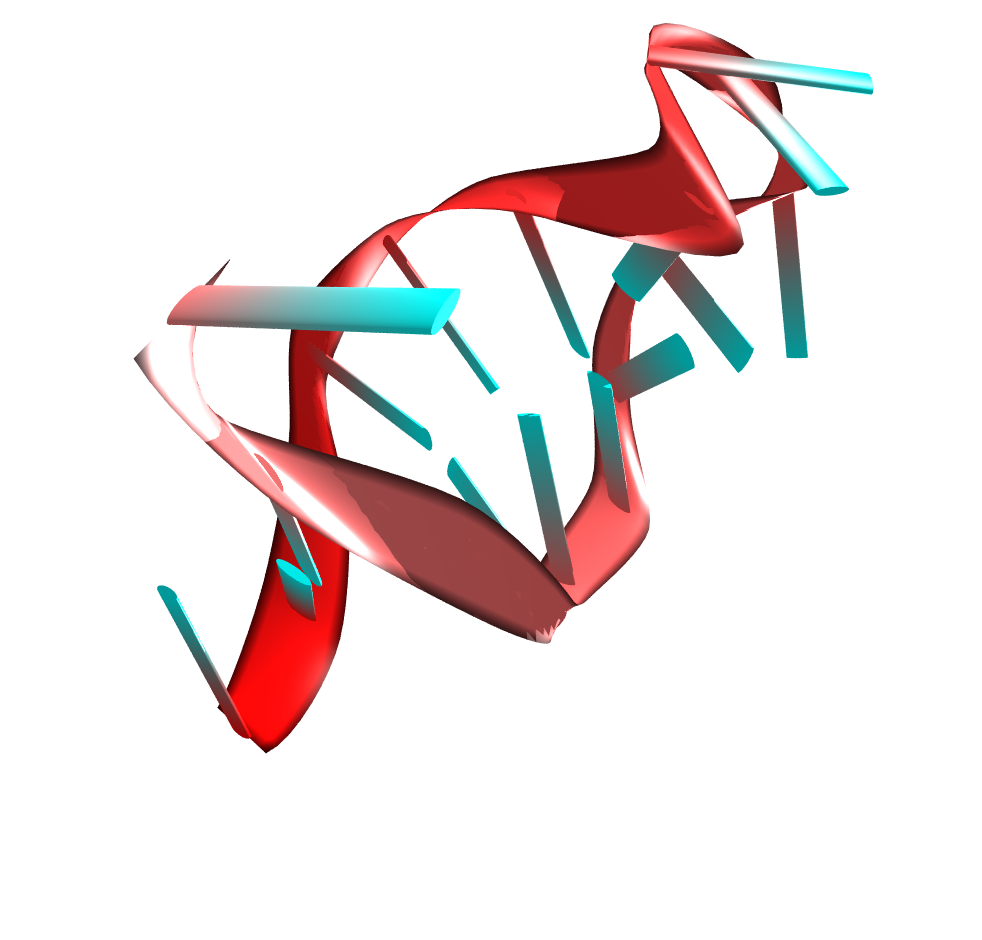
\includegraphics[width=15cm]{hairpin.png}
\label{fig:histo_MD_seq_dep}
\end{figure}

\maketitle

\section{Introduction}
\label{sec:introduction}

In this example, you will simulate a single strand of length $18$ and sequence {\tt GCGTTGCTTCTCCAACGC} at $334$ K ($\approx 61^\circ$ C) in three different ways:

\begin{enumerate}
\item with a molecular dynamics (MD) simulation of the sequence-averaged (SA) model. The input file is \texttt{inputMD}.
\item with an MD simulation of the sequence-dependent (SD) model. The input file is \texttt{inputMD\_seq\_dep}. 
\item with a Monte Carlo (MC) simulation of the SA model in which two base pairs are connected by mutual traps (i.e. additional attractive interactions between two nucleotides). The input file is \texttt{inputTRAP}.
The traps act between the pairs depicted in blue and red in the sequence G{\color{red}C}{\color{blue}G}GTTGCTTCTCCAA{\color{blue}C}{\color{red}G}C. The details of the interaction associated to the traps can be changed in the file \texttt{hairpin\_forces.dat}.
\end{enumerate}

This strand, if $T$ is sufficiently low, tends to form an hairpin with a 6-base long stem and a 6-base long loop.
The temperature has been chosen to be close to the melting temperature of such a hairpin in the SA version of the  model~\cite{ouldridge_jcp}.

This document explains how to prepare the \textit{hairpin} example (Section~\ref{sec:setup}) and how to run it (Section~\ref{sec:run}). Section~\ref{sec:results} contains results and plots extracted from the simulation output. In the following, \texttt{\$EXEC} refers to the oxDNA executable.

\section{Preparation}
\label{sec:setup}

The script \texttt{run.sh} generates the input files and runs all the three simulations, one after the other. With the default input files, each simulation, lasting $10^8$ steps by default, takes approximately one hour on a modern CPU. The default \texttt{run.sh} expects \$EXEC to be in the \texttt{../..} directory. If this is not the case, open \texttt{run.sh} and change the variable \texttt{CODEDIR} accordingly.

If you only want to generate the initial configuration, you can issue \texttt{./run.sh --generate-only}. Then you can run the simulations by yourself. The generated initial configuration files are \texttt{initial.top} (which contains the topology) and \texttt{initial.conf} (which contains positions and orientations of the nucleotides).

\section{Running the example}
\label{sec:run}

In order to run the whole example, it is sufficient to issue the command \texttt{./run.sh} (or \texttt{bash run.sh}). As described in Section~\ref{sec:setup}, you can generate the initial configuration and then run the simulations by hand. The three simulations, described in Section~\ref{sec:introduction}, can be performed issuing \texttt{\$EXEC input}, where \texttt{input} is a text file that specifies the simulation configuration. For this example, three files have been prepared: \texttt{inputMD}, \texttt{inputMD\_seq\_dep} and \texttt{inputTRAP}. Table~\ref{tbl:sim} report all the files associated to each simulations.

\begin{table}[h]
\begin{tabular}{| c | c | c | c | c | c |}
\hline
Type & input & energy file & trajectory file & last configuration file & log file\\
\hline \hline
SA model & inputMD & energy.dat & trajectory.dat & last\_conf.dat & log.dat\\
SD model & inputMD\_seq\_dep & energy\_seq\_dep.dat & trajectory\_seq\_dep.dat & last\_conf\_seq\_dep.dat & log\_seq\_dep.dat\\
SA model with traps & inputTRAP & energy\_trap.dat & trajectory\_trap.dat & last\_conf\_trap.dat & log\_trap.dat\\
\hline
\end{tabular}
\caption{Input and output files associated to each different simulation.}
\label{tbl:sim}
\end{table}


\section{Results}
\label{sec:results}

As mentioned in Section~\ref{sec:introduction}, temperature has been chosen so that the hairpin is near its melting temperature when simulated via SA model. Figure~\ref{fig:histo_MD} shows the probability distribution histogram $P(U_{HB})$ for the hydrogen-bonding (HB) energy $U_{HB}$ of the system (in simulation units~\cite{ouldridge_jcp}). Both the minimum in $P(U_{HB})$ and a direct inspection of the time series (inset) show that the hairpin is indeed near the melting temperature, since $U_{HB}$ oscillates between $0$ (no HBs) and $\approx -3.5$, which corresponds to $4-5$ hydrogen-bonded nucleotides. At this temperature the fraying effect is relevant, and therefore the last base-pair is not always formed~\cite{ouldridge_jcp}. This is clearly visible in the snapshot at the beginning of this document, in which $4$ base-pairs are formed.

\begin{figure}[h!]
\centering
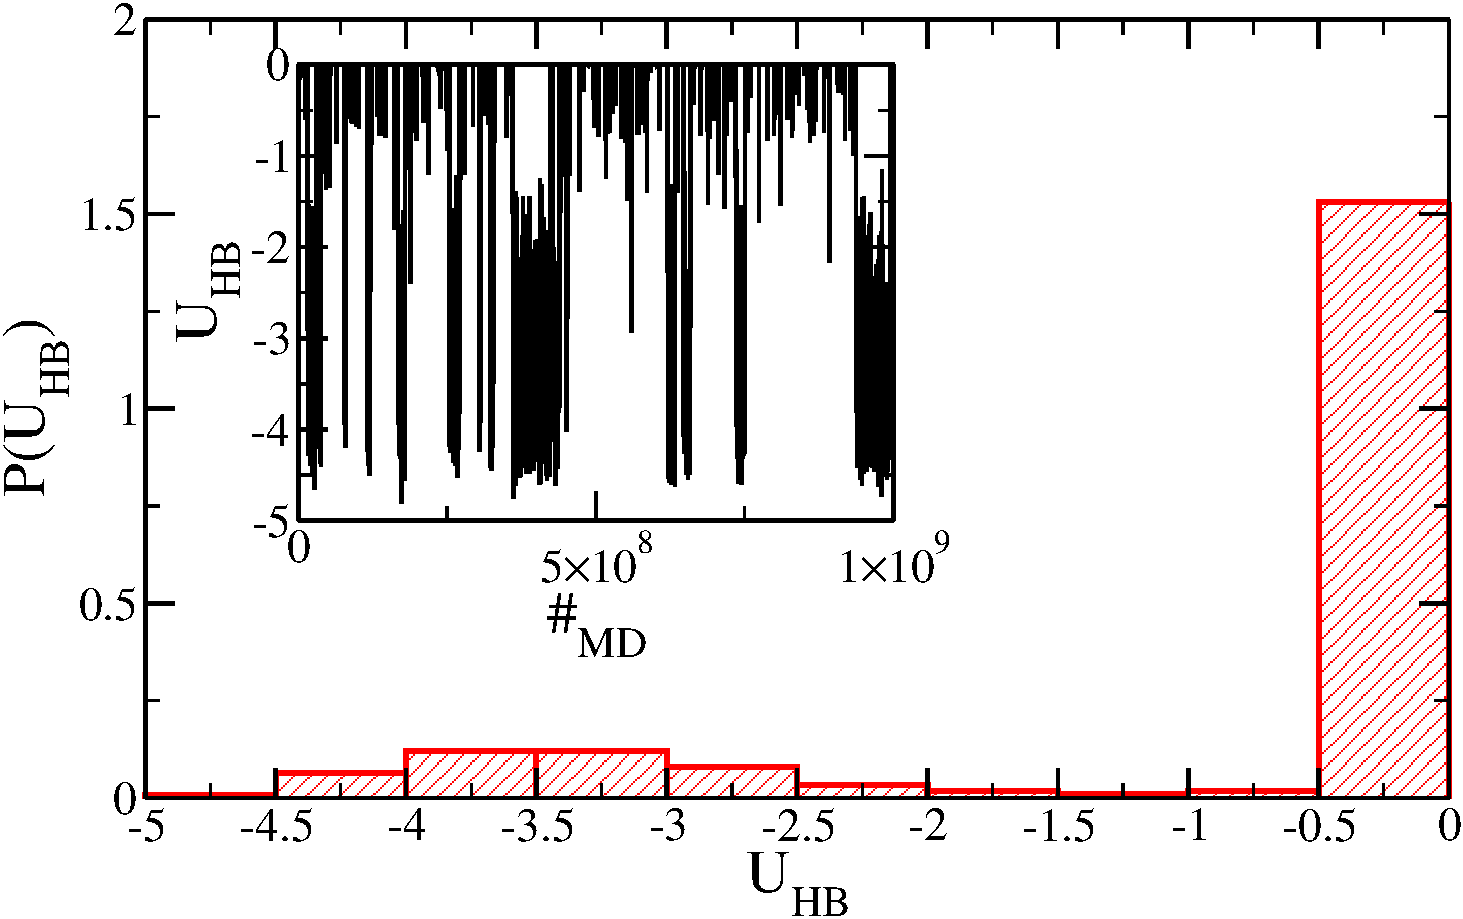
\includegraphics[width=12cm]{histo_MD.pdf}
\caption{Probability of having a hydrogen-bonding interaction energy $U_{HB}$ for the SA model. Inset: time series of the hydrogen-bonding energy (stored in the fifth column of the energy file, see Table~\ref{tbl:sim}) as a function of MD steps.}
\label{fig:histo_MD}
\end{figure}

Figure~\ref{fig:histo_MD_seq_dep} shows $P(U_{HB})$ and $U_{HB}$ for the SD hairpin. In this case, one expects a different melting temperature. Indeed, at this temperature the hairpin is nearly always in its folded conformation and the average value of $U_{HB}$ is lower than in the SA case. Although stacking interactions play a role, the major contribution to this effect is due to the presence of four \texttt{GC} only two \texttt{AT} base-pairs in the stem.

\begin{figure}[h!]
\centering
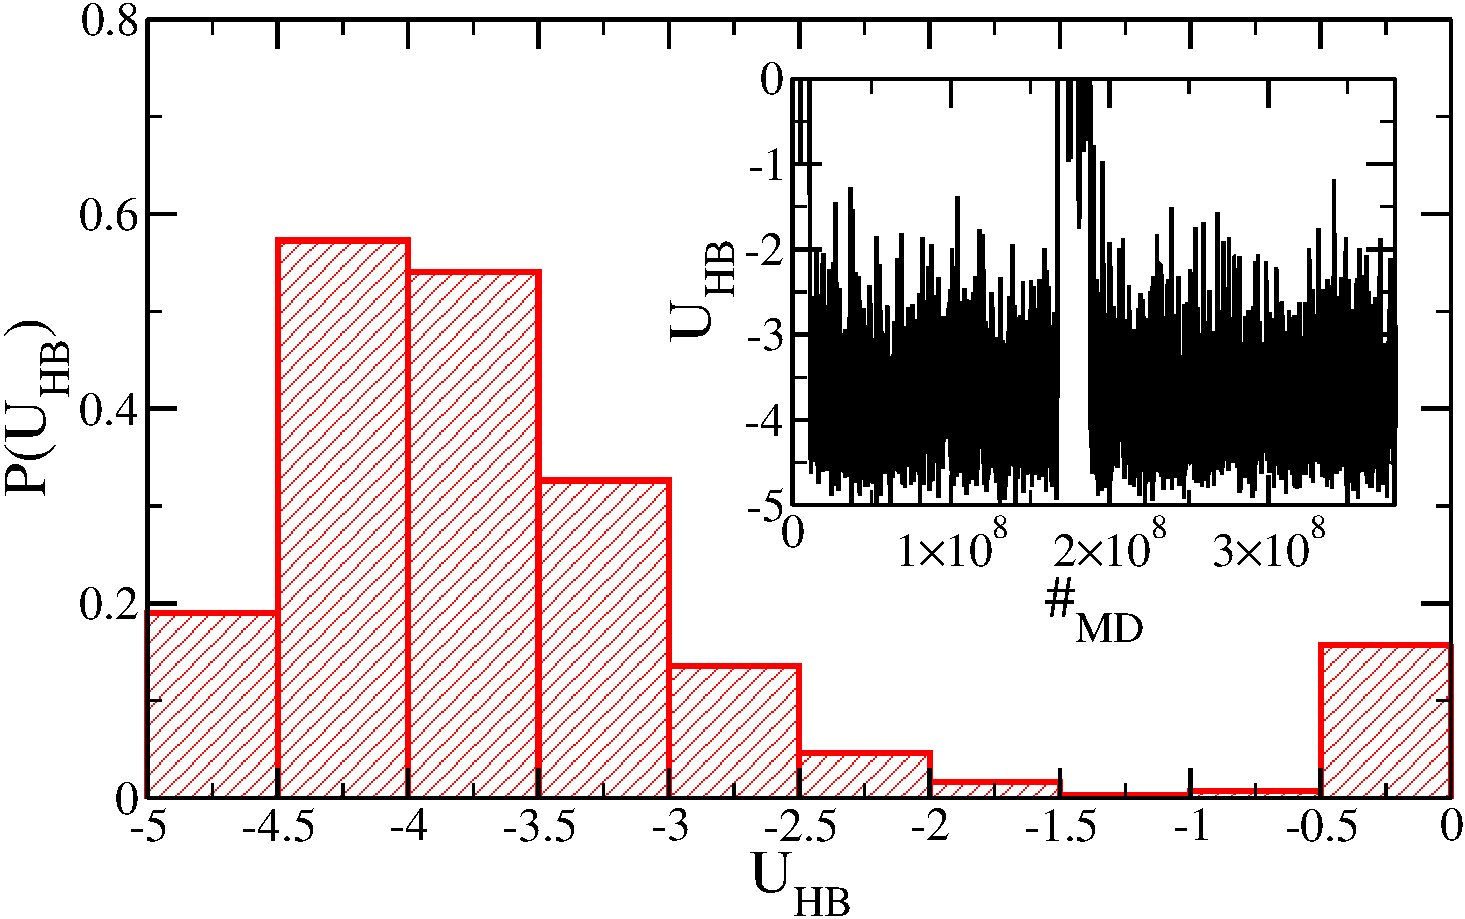
\includegraphics[width=12cm]{histo_MD_seq_dep.pdf}
\caption{Same as Figure~\ref{fig:histo_MD}, but for the SD model.}
\label{fig:histo_MD_seq_dep}
\end{figure}

If mutual traps between stem base-pairs are introduced, then the equilibrium properties of the hairpin are changed and, even if the SA model is employed, the hairpin is always (after the initial equilibration) in its folded conformation. The use of mutual traps can highly decrease the simulation time required by the folding of strands into target structures (like DNA origami or DNA constructs).

\begin{figure}[h!]
\centering
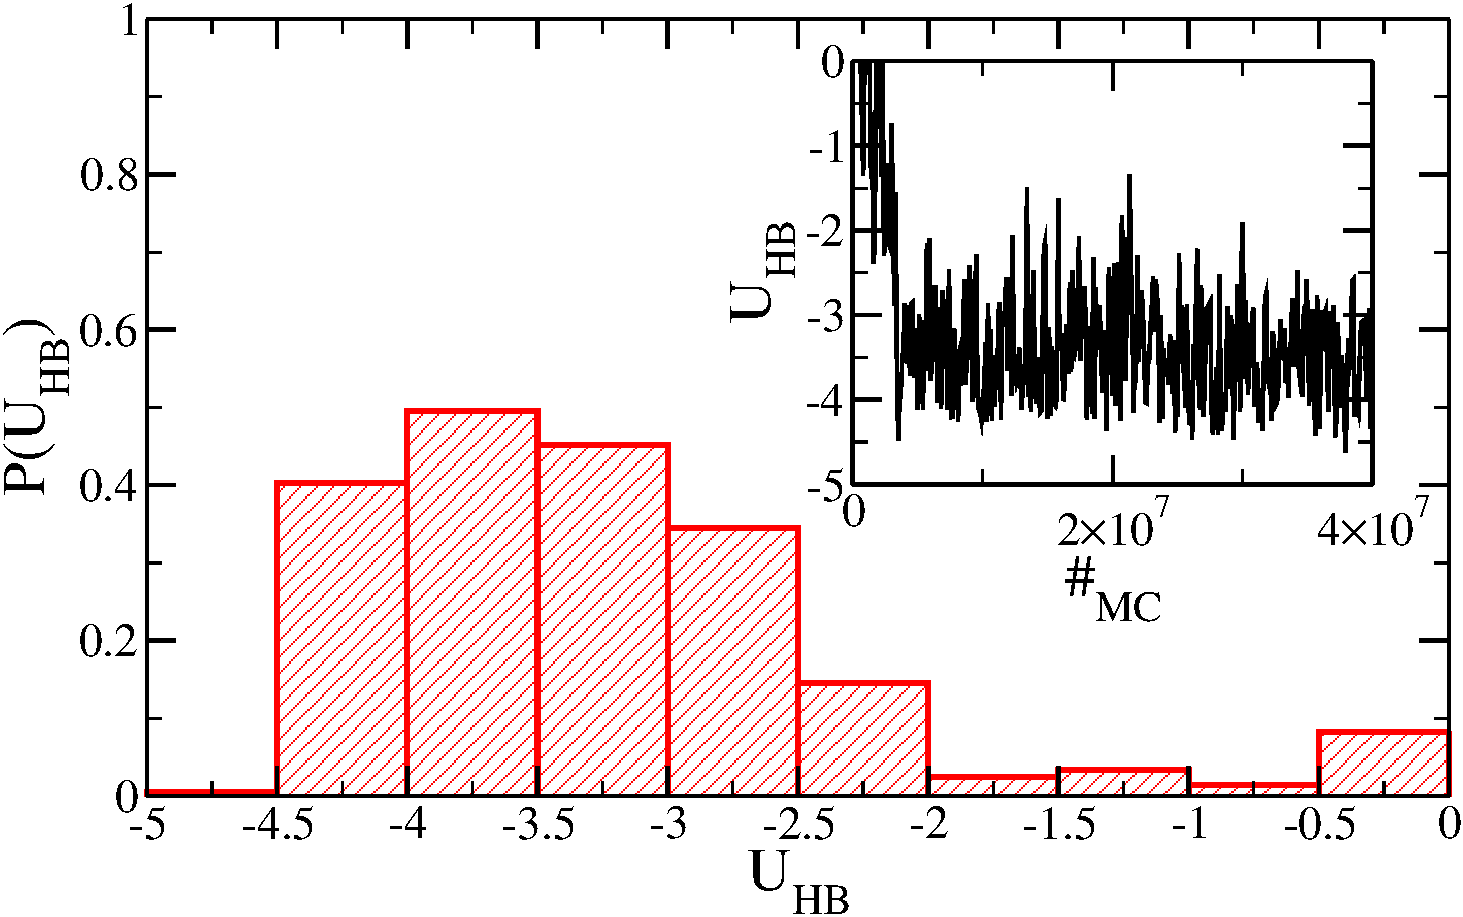
\includegraphics[width=12cm]{histo_TRAP.pdf}
\caption{Same as Figure~\ref{fig:histo_MD}, but for the system with mutual traps. Time is expressed in Monte Carlo sweeps.}
\label{fig:histo_TRAP}
\end{figure}

\newpage

\begin{thebibliography}{10}

\bibitem{ouldridge_jcp}
T.~E. Ouldridge, A.~A. Louis, and J.~P.~K. Doye, {\em J. Chem. Phys.}, {\bf
  134}(8), 085101 (2011). Structural, mechanical, and thermodynamic properties
  of a coarse-grained dna model.

\end{thebibliography}

\end{document}